\section{Small Data sets}
\label{sec: small_data_sets}
\begin{figure}[!t]
	\centering
	\vspace{0.5mm}
	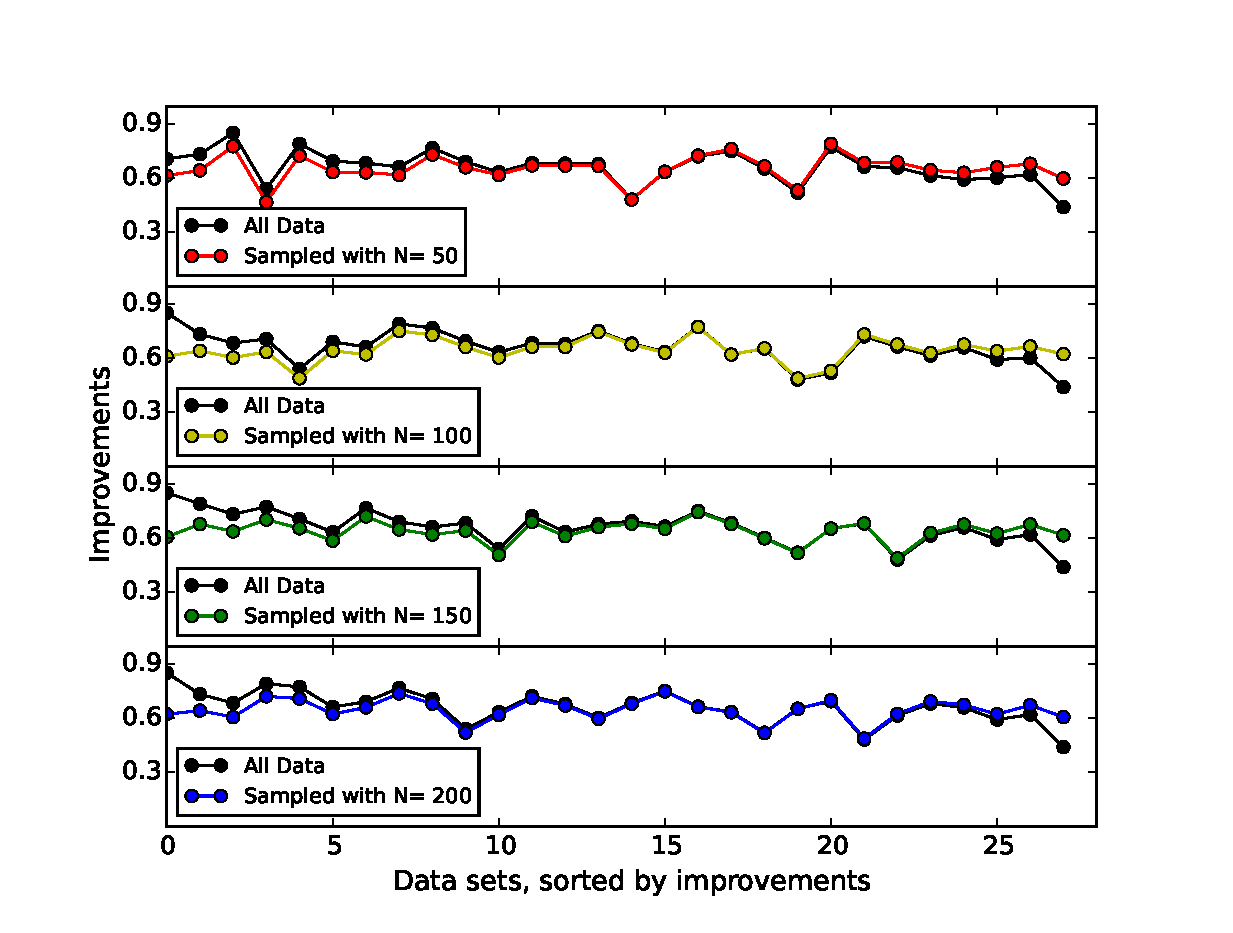
\includegraphics[width=4.5in]{Figures/raleigh/sampled.eps}
	\caption{Distribution of metrics (matching score=0.91)
	from ant-1.3$\Rightarrow$ar5 (AUC=0.946).}
	\label{fig:best_dist}
\end{figure}

% \begin{figure}[!t]
% \begin{center}
% \includegraphics[width=1.5in]{./eps/improvements_precision.eps}\includegraphics[width=1.5in]{./eps/improvements_F.eps}
%  \end{center}
% \caption{Deltas in performance  seen in \tab{precisionbars} (left)
% and \tab{fbars} (right) between tuned and untuned learners. Tuning improves performance when the deltas are above zero.}\label{fig:deltas}
%  \end{figure}